\chapter{Analysis}

- Scenarios
-- Redirect when full
-- Select router peer, show for almost gobbel


- Hard limits
    - ttl
    - stream baum vs minimal spanning tree
        - histogram

- Discussion
- scaling further
    - dht

- nucleus scenarios
    - gobble
    - eclipsed group re–joining
    - router lost
    - glare problem: two peers try to open same connection
        - circuit glare, aka dual seizure like in phone systems
        - see \cite[pp. 194-194]{signaling-systems-book}


- Security
    - Eclipse attack
    - Sybil attack
    - ... see S/Kademlia

- Signalling
    - geographical cluster selection


Random Quotes:
\say{Analysis of a P2P system by Saroiu et al. [3] show that the longer a node has been up, the more likely it is to remain up for another hour.}(http://gleamly.com/article/introduction-kademlia-dht-how-it-works). IPFS bitswapping auch da hinschreiben

\section{Analysing small scenarios}
\subsection{Genesis}

\begin{figure}[htb!]
  \centering
    \subfloat[]{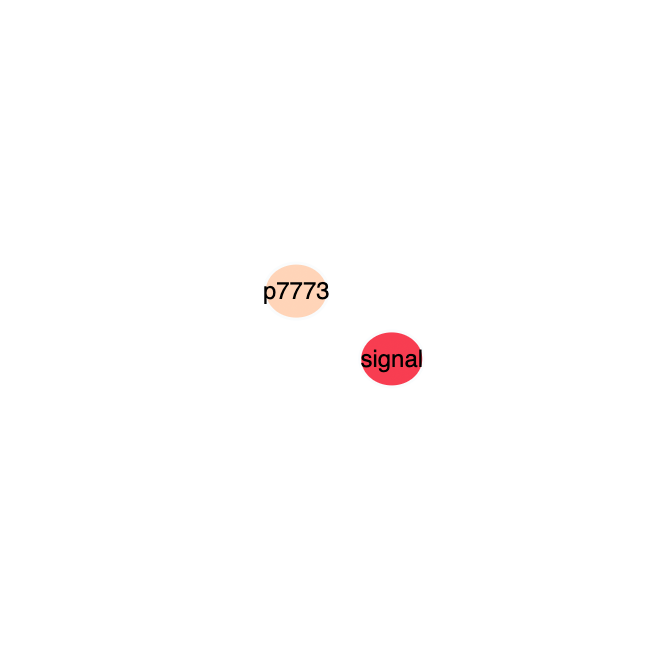
\includegraphics[width=0.33\textwidth]{graphics/analysis/mini-scenarios/become-router/1.png} 
    \label{fig:filmstrips-genesis-a}}
    \subfloat[]{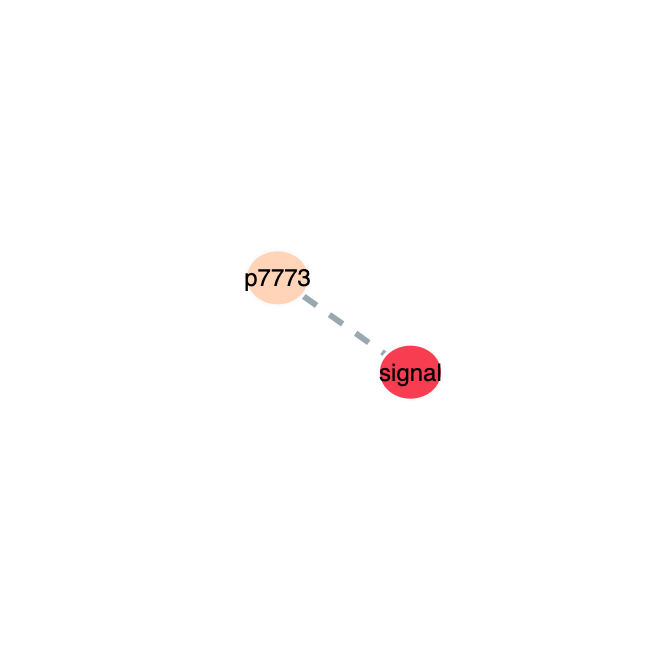
\includegraphics[width=0.33\textwidth]{graphics/analysis/mini-scenarios/become-router/2.png} \label{fig:filmstrips-genesis-b}}
	\subfloat[]{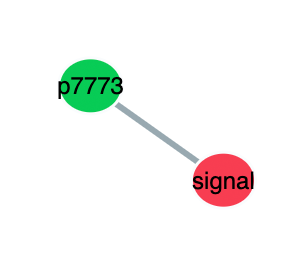
\includegraphics[width=0.33\textwidth]{graphics/analysis/mini-scenarios/become-router/3.png} \label{fig:fig:filmstrips-genesis-c}}
	\caption{Join network as first peer}
\label{fig:overlay-topologies}
\end{figure}
\subsection{Join network \rom{1}}

\begin{figure}[htb!]
  \centering
    \subfloat[]{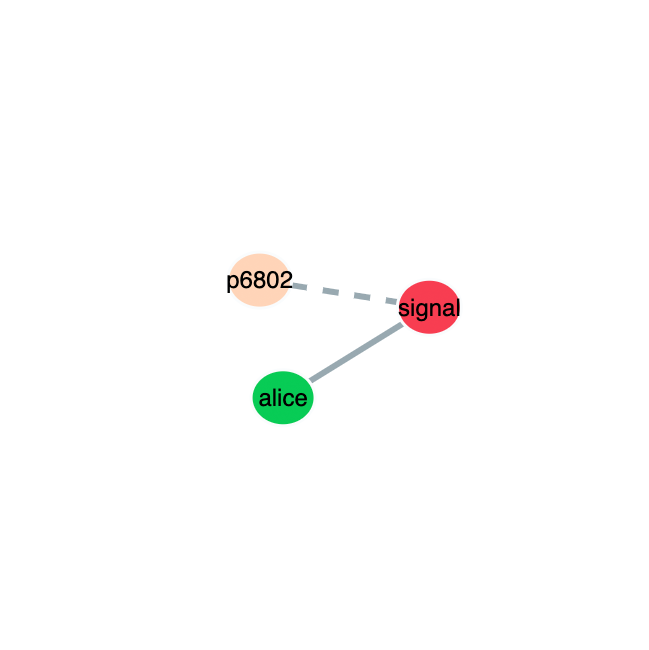
\includegraphics[width=0.25\textwidth]{graphics/analysis/mini-scenarios/join-network/1.png} \label{fig:filmstrips-join-a}}
    \subfloat[]{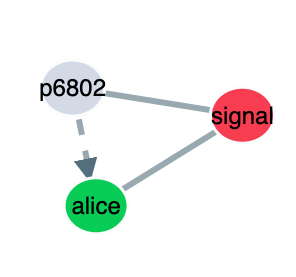
\includegraphics[width=0.25\textwidth]{graphics/analysis/mini-scenarios/join-network/2.png} \label{fig:filmstrips-join-b}}
	\subfloat[]{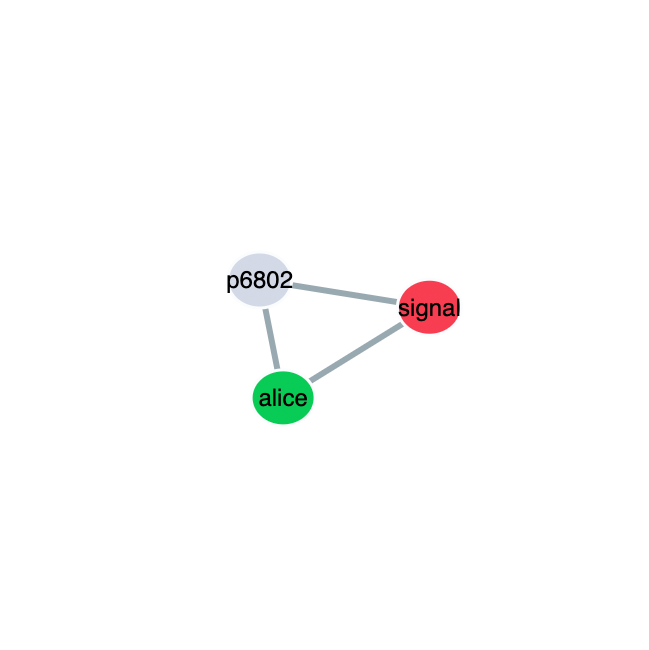
\includegraphics[width=0.25\textwidth]{graphics/analysis/mini-scenarios/join-network/3.png} \label{fig:filmstrips-join-c}}
	\subfloat[]{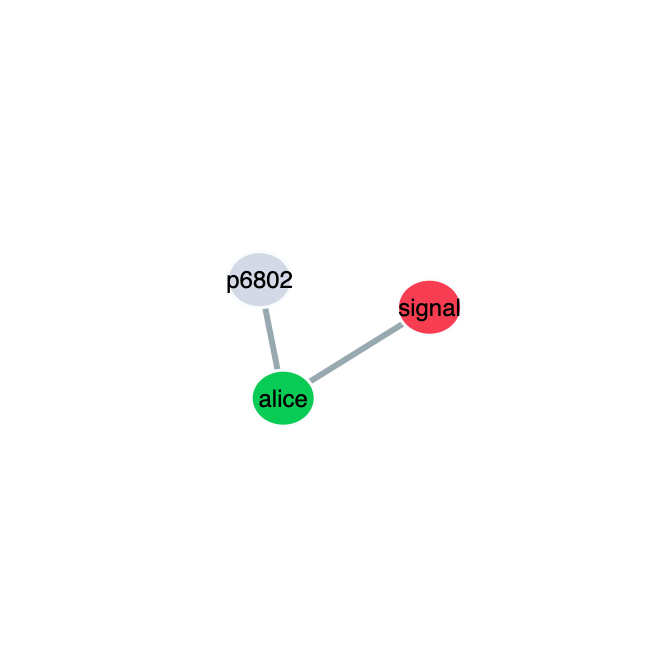
\includegraphics[width=0.25\textwidth]{graphics/analysis/mini-scenarios/join-network/4.png} \label{fig:filmstrips-join-d}}
	\caption{Join network as second peer}
\label{fig:filmstrips-join}
\end{figure}

In this scenario a second peer is joining the network. As described in the in the \textit{Genesis} scenario it opens a connection to the \signal peer (\vref{fig:filmstrips-join-a}). This time the \signal peer already knows a \router peer—\alice. Therefore, it only upgrades the \newbie peer to the role \peer. Also it sends a \peerUpdate to the new peer in order to let it update its peer table. 

A peer with the role \peer has always the desire to satisfy its connection goal.
Thus, its next intention is to open connections to as many peers as it knows, until its connection goal is satisfied. As it only knows the reported peer \alice it is trying to connect to her by sending a connection offer via the \signal peer (\vref{fig:filmstrips-join-b}).

\alice has connections available, hence she is accepting the connection offer with an answer, that is again delivered via the \signal. As soon as the new peer receives the answer, it establishes the connection to \alice (\vref{fig:filmstrips-join-c}).

In the last step it closes the connection to the \signal peer because it knows a peer with the role \router (\vref{fig:filmstrips-join-d}).


\subsection{Join network but router is already full of capacity}

\begin{figure}[htb!]
  \centering
    \subfloat[]{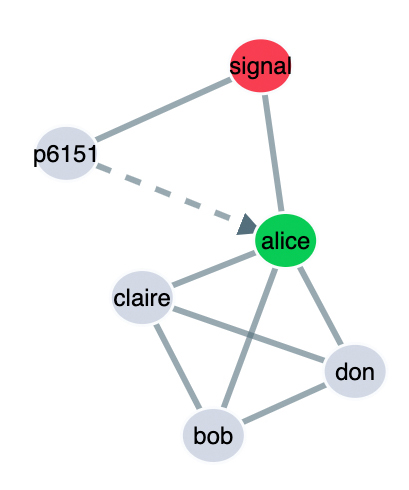
\includegraphics[width=0.33\textwidth]{graphics/analysis/mini-scenarios/router-full-redirect/1.jpg} \label{fig:filmstrips-redirect-a}}
    \subfloat[]{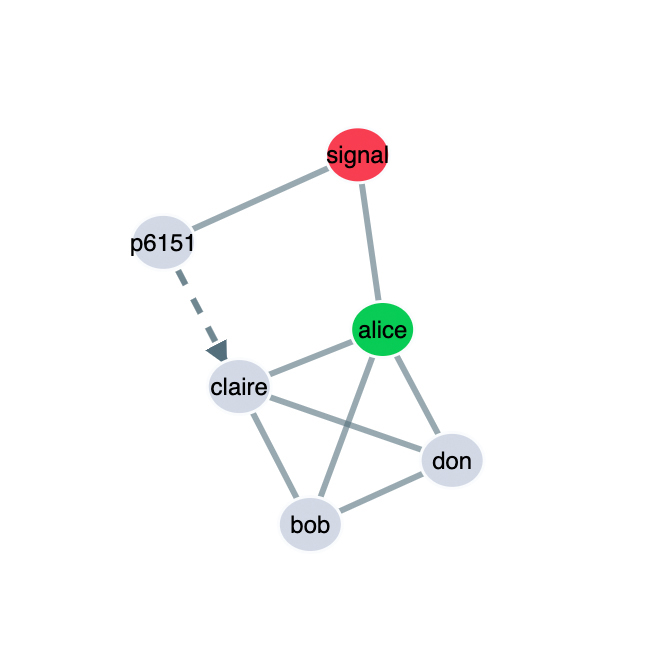
\includegraphics[width=0.33\textwidth]{graphics/analysis/mini-scenarios/router-full-redirect/2.jpg} \label{fig:filmstrips-redirect-b}}
	\subfloat[]{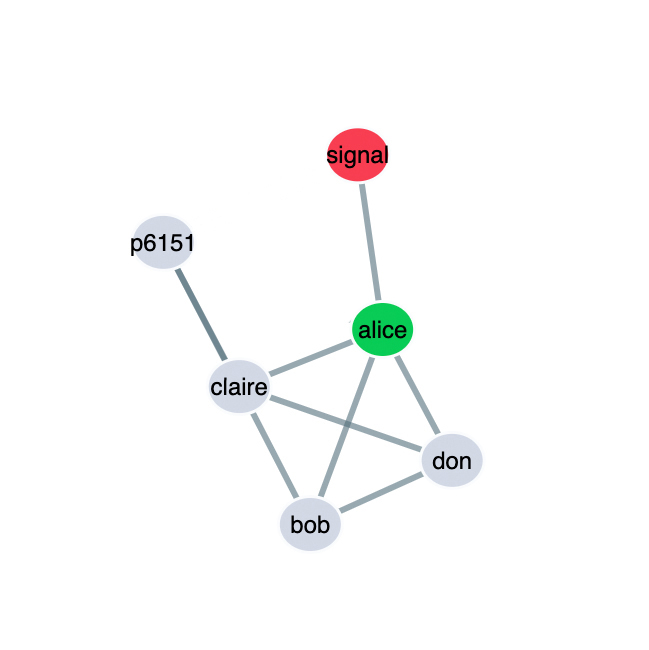
\includegraphics[width=0.33\textwidth]{graphics/analysis/mini-scenarios/router-full-redirect/3.jpg} \label{fig:filmstrips-redirect-c}}
	\caption{Join network peer}
\label{fig:overlay-topologies}
\end{figure}
\subsection{Bottleneck prevention}

\begin{figure}[htb!]
  \centering
    \subfloat[]{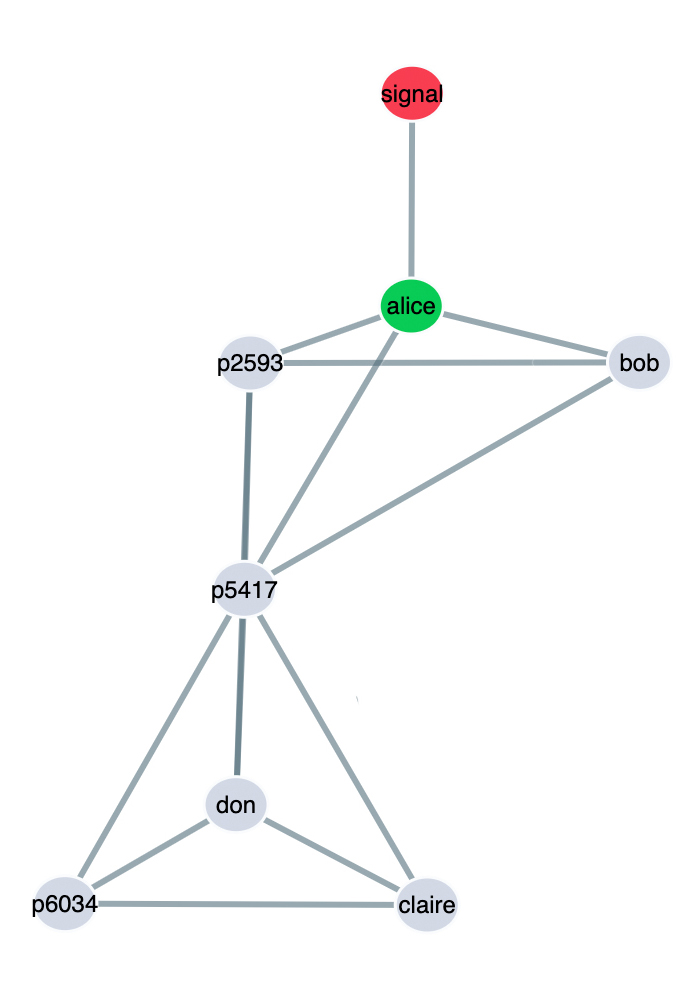
\includegraphics[width=0.33\textwidth]{graphics/analysis/mini-scenarios/bottleneck-prevention/1.jpg} \label{fig:filmstrips-bottleneck-prevention-a}}
    \subfloat[]{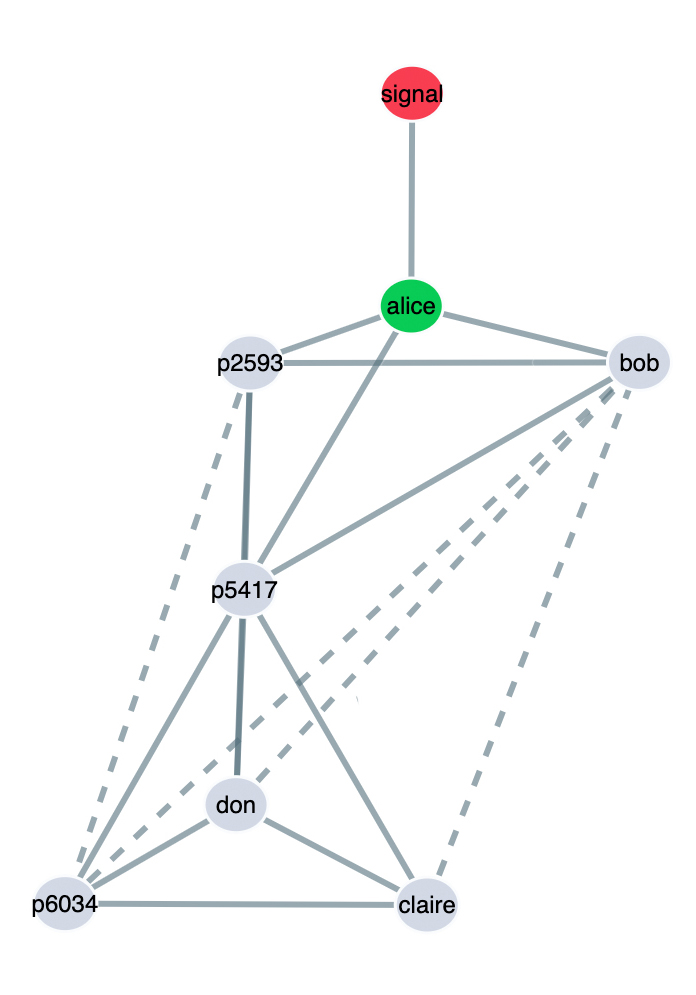
\includegraphics[width=0.33\textwidth]{graphics/analysis/mini-scenarios/bottleneck-prevention/2.jpg} \label{fig:filmstrips-bottleneck-prevention-b}}
	\subfloat[]{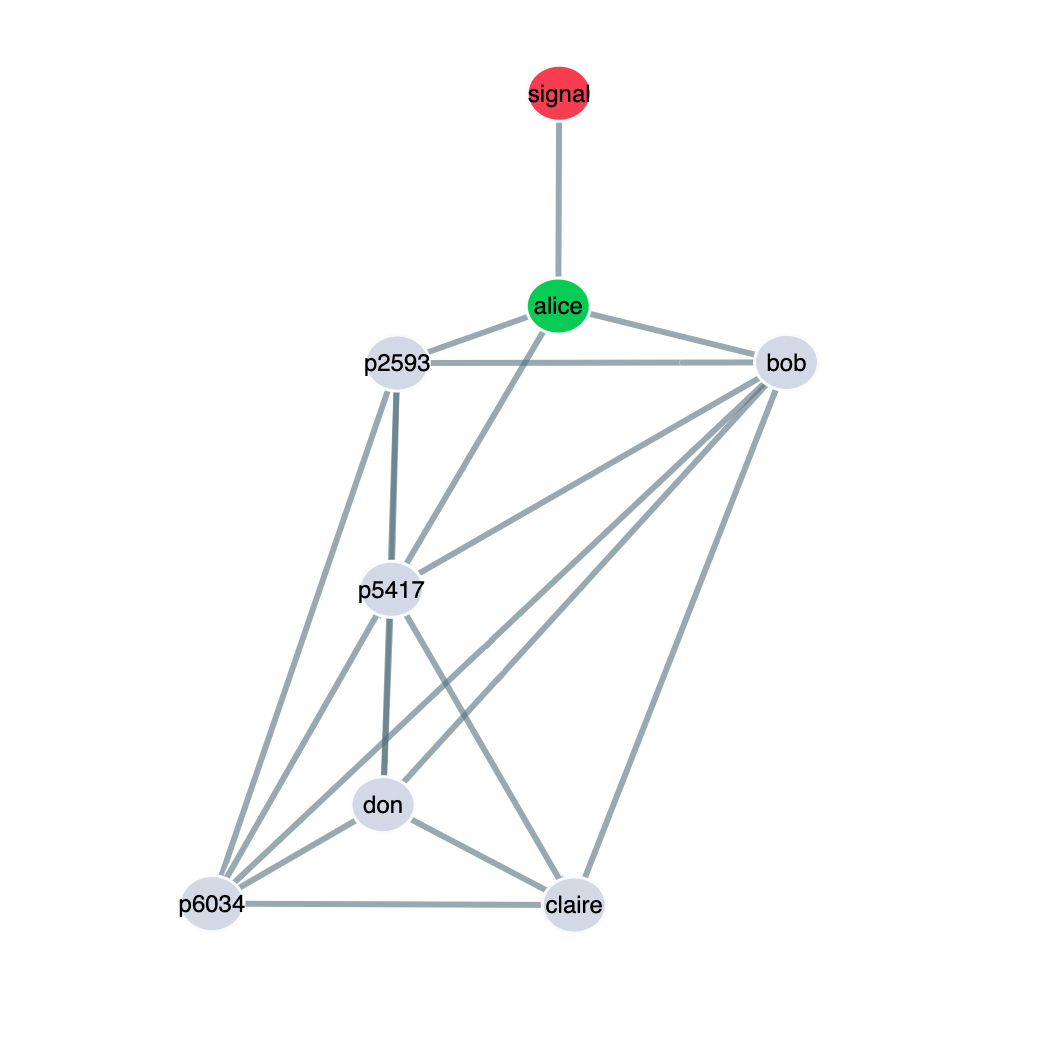
\includegraphics[width=0.33\textwidth]{graphics/analysis/mini-scenarios/bottleneck-prevention/3.jpg} \label{fig:filmstrips-bottleneck-prevention-c}}
	\caption{Preventing a bottleneck}
\label{fig:overlay-topologies}
\end{figure}
\subsection{Send message}

\begin{figure}[htb!]
  \centering
    \subfloat[]{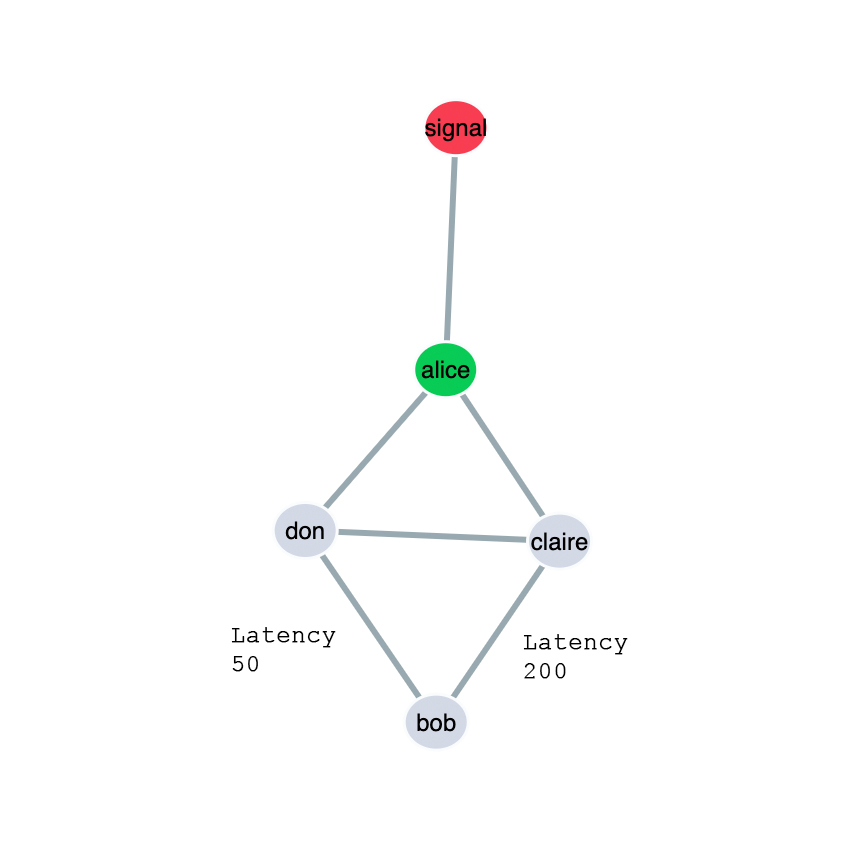
\includegraphics[width=0.25\textwidth]{graphics/analysis/mini-scenarios/send-message/1.jpg} \label{fig:filmstrips-send-message-a}}
    \subfloat[]{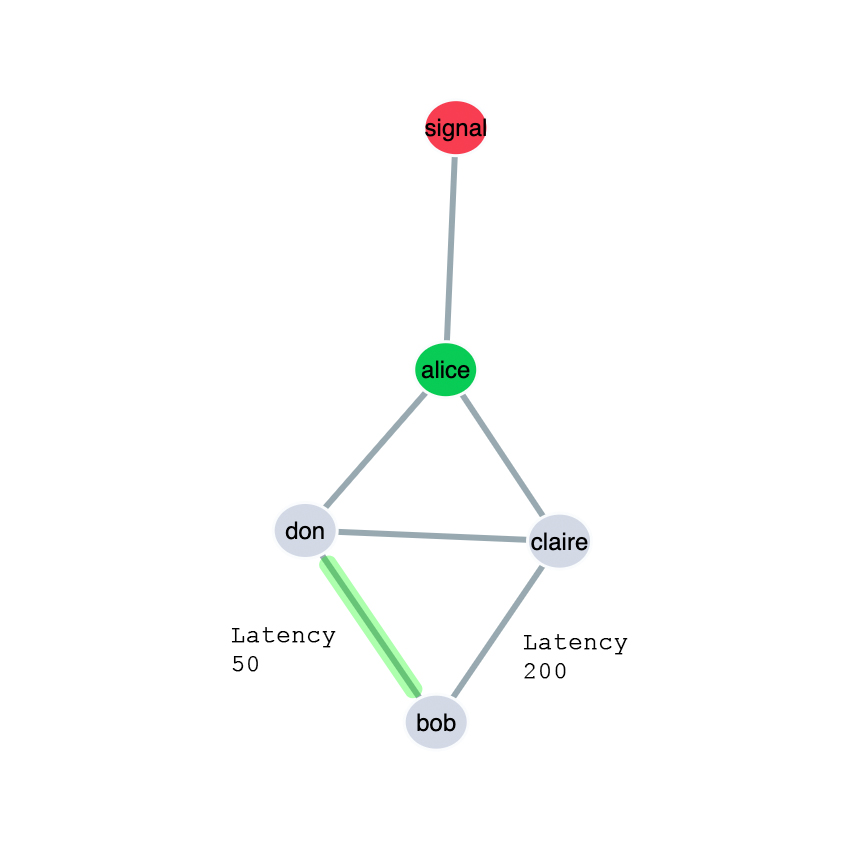
\includegraphics[width=0.25\textwidth]{graphics/analysis/mini-scenarios/send-message/2.jpg} \label{fig:filmstrips-send-message-b}}
	\subfloat[]{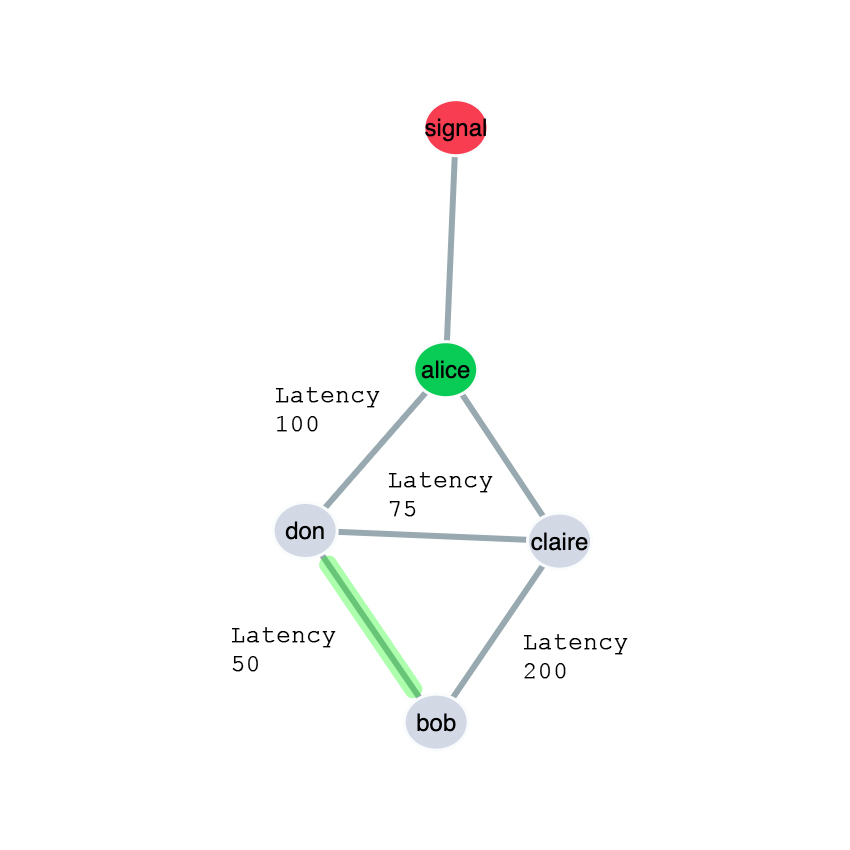
\includegraphics[width=0.25\textwidth]{graphics/analysis/mini-scenarios/send-message/3.jpg} \label{fig:filmstrips-send-message-c}}
	\subfloat[]{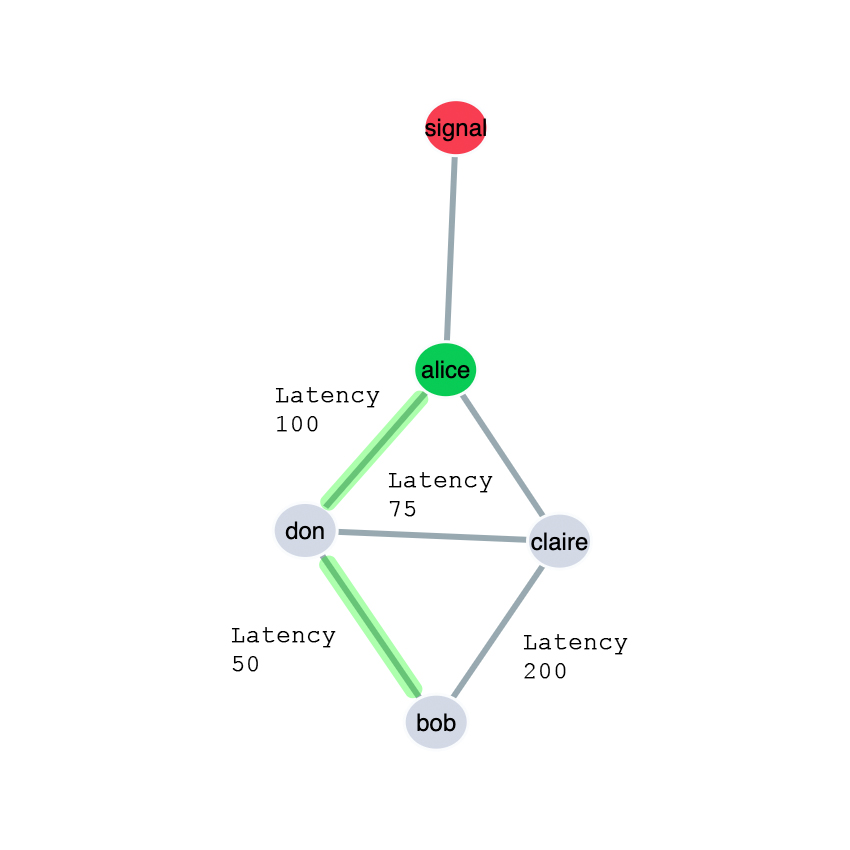
\includegraphics[width=0.25\textwidth]{graphics/analysis/mini-scenarios/send-message/4.jpg} \label{fig:filmstrips-send-message-d}}
	\caption{Path of a message}
\label{fig:overlay-topologies}
\end{figure}
\subsection{Broadcast}

\begin{figure}[htb!]
  \centering
    \subfloat[]{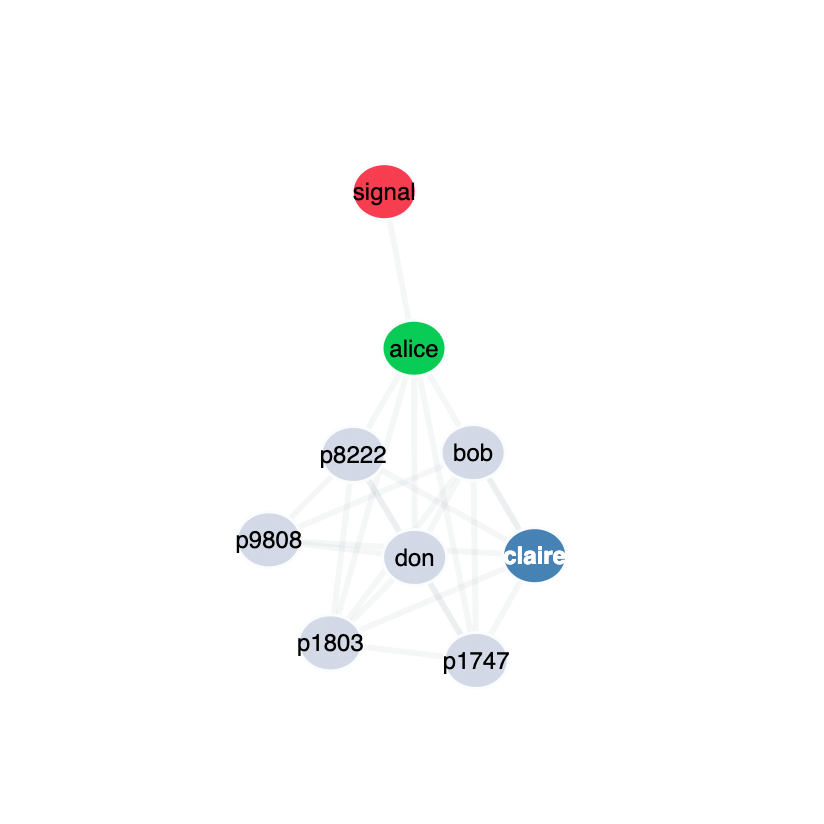
\includegraphics[width=0.25\textwidth]{graphics/analysis/mini-scenarios/stream/1.png} \label{fig:filmstrips-broadcast-a}}
    \subfloat[]{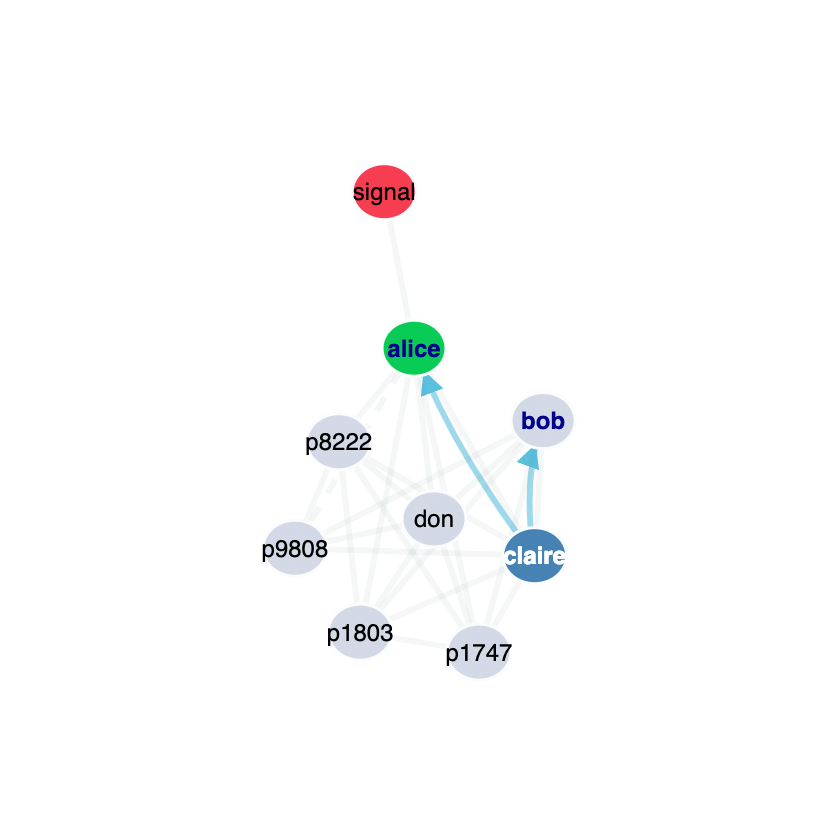
\includegraphics[width=0.25\textwidth]{graphics/analysis/mini-scenarios/stream/2.png} \label{fig:filmstrips-broadcast-b}}
	\subfloat[]{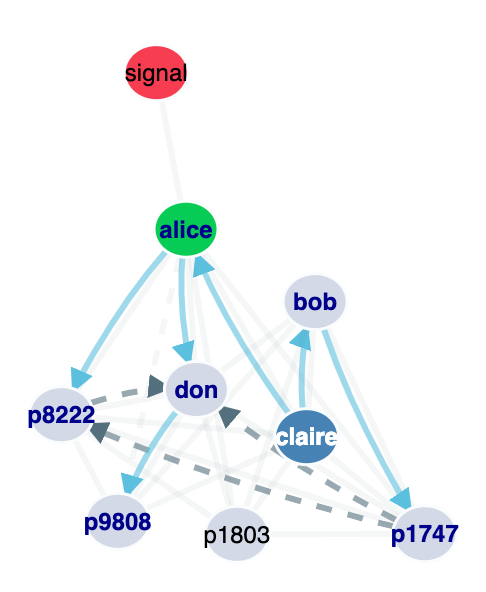
\includegraphics[width=0.25\textwidth]{graphics/analysis/mini-scenarios/stream/3.png} \label{fig:filmstrips-broadcast-c}}
	\subfloat[]{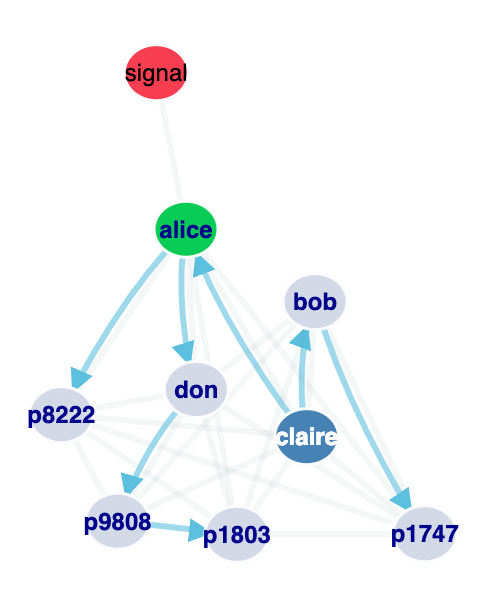
\includegraphics[width=0.25\textwidth]{graphics/analysis/mini-scenarios/stream/4.png} \label{fig:filmstrips-broadcast-d}}
	\caption{Broadcasting tree creation}
\label{fig:overlay-topologies}
\end{figure}
\newpage
\input{content/6-analysis/2-meshing.tex}
\newpage
\section{Streaming Analysis}

\subsection{Topology}

Since video streams over \gls{webrtc} connections decrease in quality per hop, as discussed in \vref{TOOD}, an optimal streaming topology would would be a \textit{perfect k–ary tree}, given nodes can upload $k$ streams simultaneously. A perfectly balanced binary tree, for example, would be the optimal streaming topology for $k=2$.

As the streaming topology is built on the collective knowledge of the overlay network, it depends heavily on the state the overlay mesh has reached at the point the stream is started. It must also be considered, that the streaming tree is constructed in the two phases detailed in \vref{TODO}. The push phase aims at achieving availability fast and does not regard tree balance.
It is also important to note, that due to node churn, the stream topology can change unexpectedly as nodes try to re–acquire a connection to a source provider.

The quality of the streaming topology is inspected in a churn–free simulation setup. Given a scenario of $n=100$ nodes and $t=1500$ ticks a stream is automatically started at $t_{500}$. The network constructs its stream topology and the active stream connections are queried at the end of the scenario. The topology is traversed and the distance to the stream source is extracted from every node. For simplicity, the connections are handled unweighted and just the hop count is considered.
Using different random seeds, multiple runs are averaged using the mean node count per distance.

\vref{fig:streaming-topology-histogram} shows the results of the hop distribution for streaming topologies for $k=2$ and $k=3$. For comparison, the histogram also shows the distribution in an optimal binary and ternary tree given $n=100$ nodes.

\begin{figure}
\centering
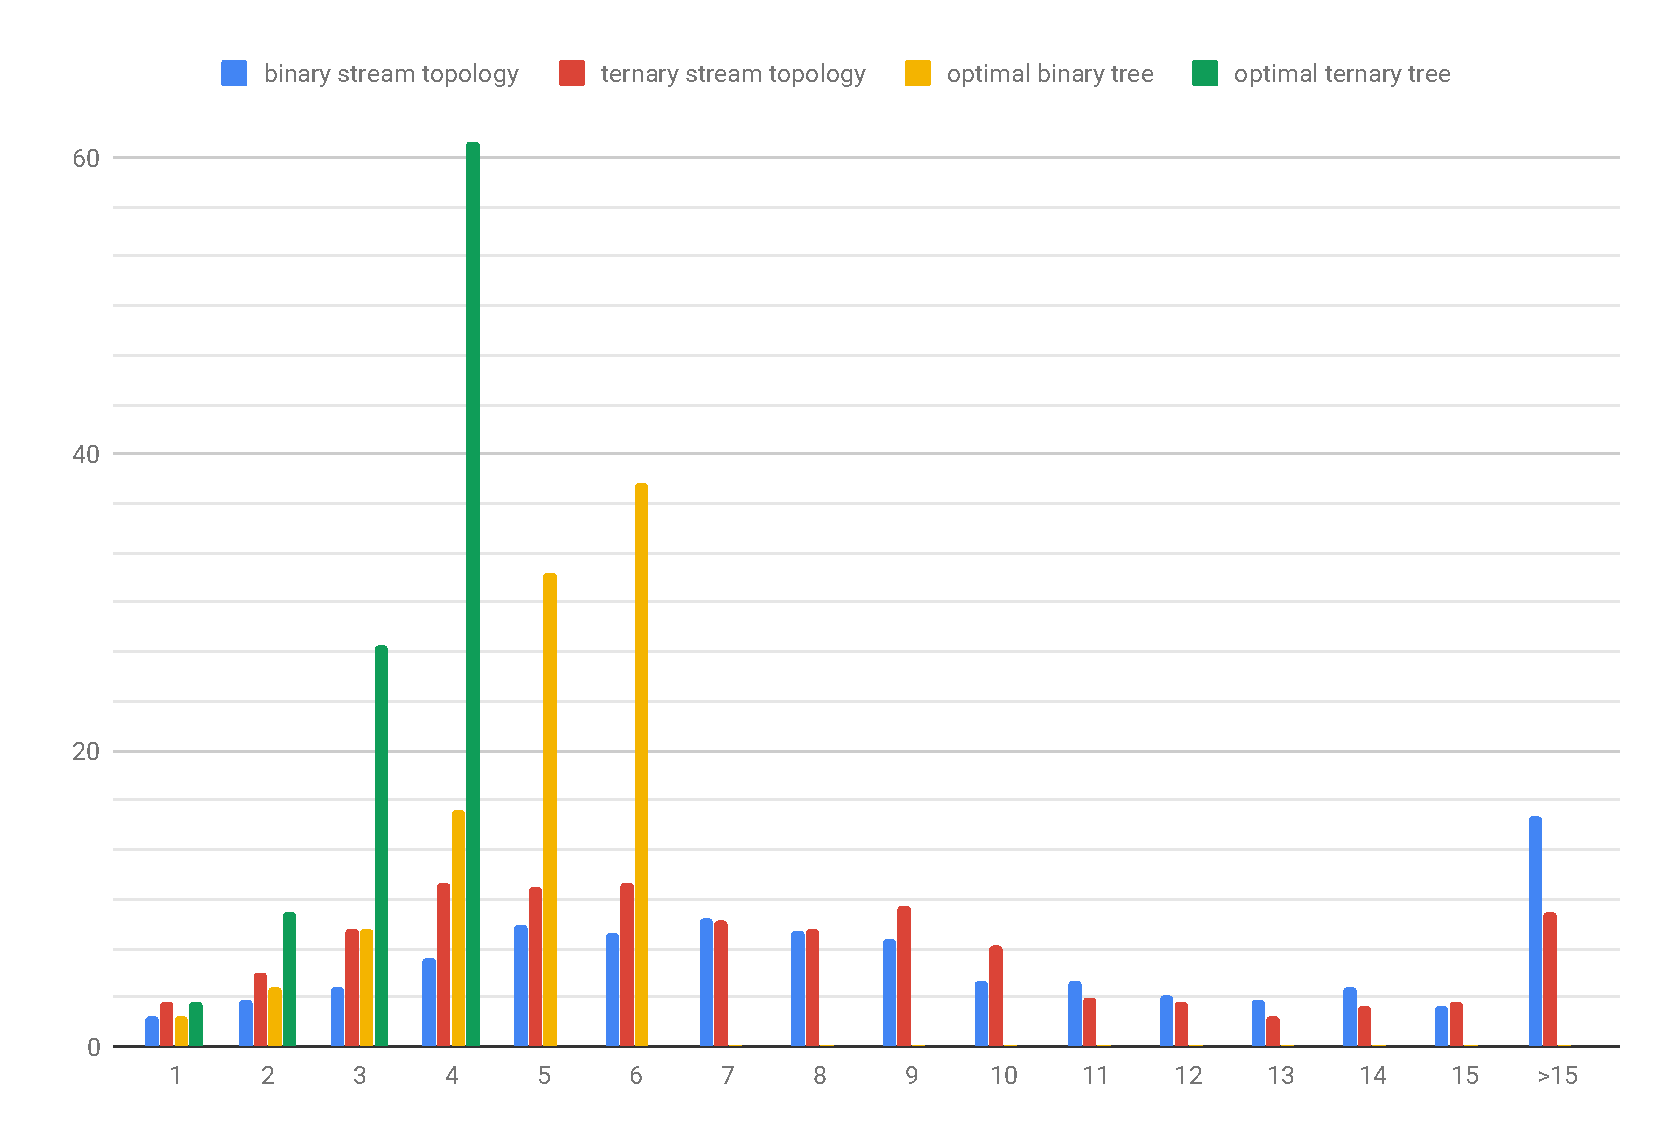
\includegraphics[width=1\textwidth]{graphics/analysis/streaming-topology-histogram.pdf}
\caption{Stream consumers per distance from stream source}
\label{fig:streaming-topology-histogram}
\end{figure}

It is evident, that the trees constructed by the overlay mesh are far from the perfectly balanced trees. A binary tree with $n=100$ nodes would not exhibit hop distances beyond $6$ and a ternary tree would not exceed distances of $4$. The respective streaming trees show a much broader distribution. The spikes caused behind the quadratic/cubic function of the optimal trees, are not to be found in the stream topologies. Yet, half the nodes exceed $8$ connection hops for $k=2$ and half the nodes for $k=3$ are above $6$ connections away from the source.

This non–optimal distribution can be explained by collisions during the push phase. As multiple nodes in the same radius around the stream source receive the channel, they try to push it out to their most reliable neighbour. However, chances are, their own best neighbour is also the choice of some other node on the same radius. As a result, this popular choice receives two connection offers, accepts only one and leaves the other offerer as a leaf node in the tree. While this is not a desirable state, the topology can self–heal during the pull phase. As nodes join or become interested in the channel, they will seek providers and can attach to the aforementioned leaf node.

So, in a second experiment, a more realistic scenario is set up. Nodes are not instantiated at once, but keep joining at a rate of $1/t$ to a total number of $n=50$. After half the nodes have joined the mesh, the stream is automatically started. \vref{fig:streaming-later-join} shows how the hop distances are distributed when nodes are continuously joining instead of being initiated before the stream start.

\begin{figure}
\centering
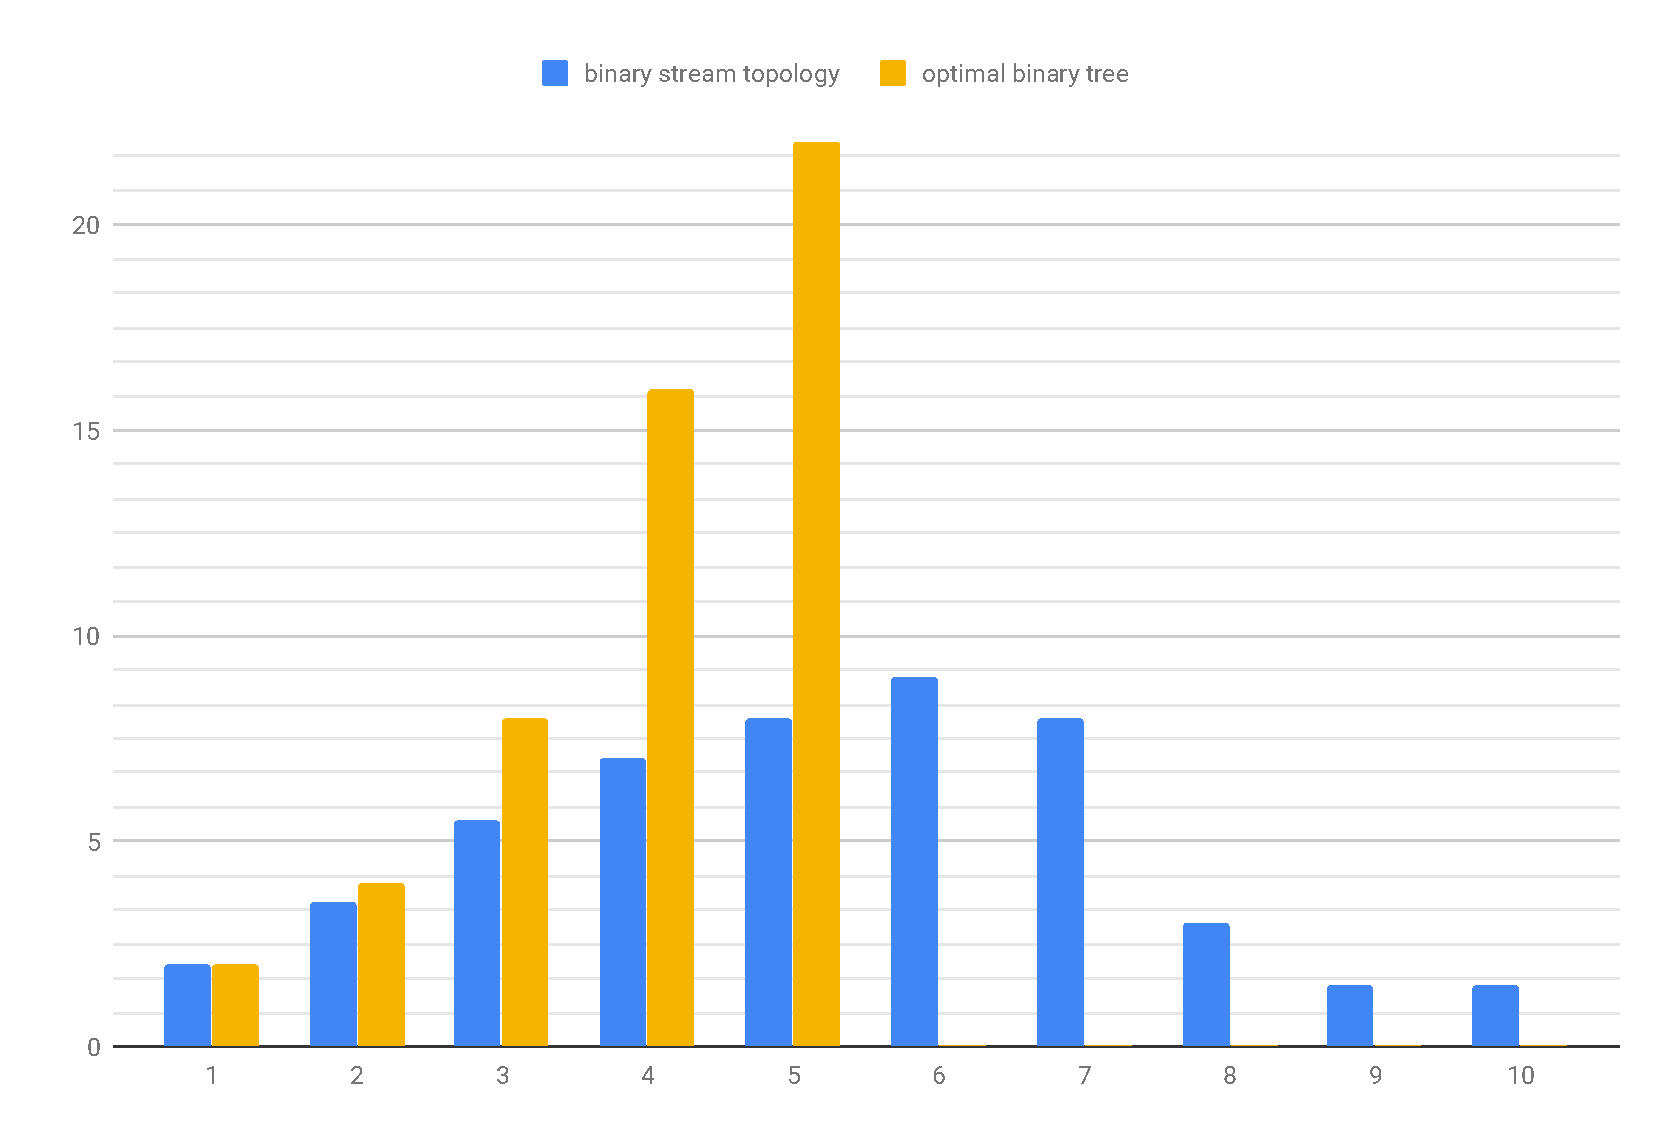
\includegraphics[width=1\textwidth]{graphics/analysis/streaming-topology-continuous-histo.pdf}
\caption{Stream consumer distance in continuous join rate scenario}
\label{fig:streaming-topology-continuous-histo}
\end{figure}

In summary, the streaming topology is heavily dependent on the underlying mesh size and structure. To cope with larger numbers of stream consumers, the system would have to perform tree optimisation. Whether this is feasible, however, depends on the application dynamics. If video channels are long–lasting and audiences are large, it would be worthwhile. If video channels are only alive a few minutes and audiences are usually small, tree optimisation would not be worth the extra negotiation effort.

\newpage
